\documentclass{article}
\usepackage{amsmath, amssymb, graphicx, geometry, tikz, array, booktabs, enumitem, listings, xcolor, fancyhdr, float, subcaption, hyperref}

\title{Module 6: Maximizing the Margin of a Linear Classifier\\(Support Vector Machines)}
\author{Machine Learning Course}
\date{}

\begin{document}

\maketitle
\tableofcontents
\newpage

\section{Introduction to Support Vector Machines}

\subsection{From Perceptron to Maximum-Margin Classifiers}
In the previous lecture, we explored the Perceptron algorithm, which finds a linear decision boundary that correctly classifies all training examples (assuming the data is linearly separable). However, the Perceptron algorithm has a key limitation: it can find any linear separator that works, but it doesn't necessarily find the "best" one.

This raises an important question: Among all possible linear separators, which one should we choose? Support Vector Machines (SVMs) provide a principled answer to this question by finding the linear separator that maximizes the margin between the two classes.

\subsection{Motivation for Maximum-Margin Classification}
Why should we care about maximizing the margin? There are several compelling reasons:

\begin{itemize}
    \item \textbf{Generalization}: A classifier with a larger margin is likely to generalize better to unseen data
    \item \textbf{Robustness}: Maximum-margin classifiers are more robust to small perturbations in the data
    \item \textbf{Theoretical guarantees}: The margin is directly related to bounds on the generalization error
    \item \textbf{Uniqueness}: Unlike the Perceptron, which can find many different solutions, the maximum-margin classifier is unique (for linearly separable data)
\end{itemize}

\section{Review of Linear Classification}

\subsection{The Perceptron Algorithm}
Let's briefly review the Perceptron algorithm:

\fbox{
\begin{minipage}{\dimexpr\textwidth-2\fboxsep-2\fboxrule\relax}
\textbf{The Perceptron Algorithm}
\begin{enumerate}
    \item Initialize $\mathbf{w} = \mathbf{0}$ and $b = 0$
    \item Keep cycling through the training data $(\mathbf{x}, y)$:
    \begin{enumerate}
        \item If $y(\mathbf{w} \cdot \mathbf{x} + b) \leq 0$ (i.e., point misclassified):
        \begin{enumerate}
            \item $\mathbf{w} = \mathbf{w} + y\mathbf{x}$
            \item $b = b + y$
        \end{enumerate}
    \end{enumerate}
\end{enumerate}
\end{minipage}
}

\subsection{Perceptron Convergence}
The Perceptron algorithm has an important convergence guarantee:

\fbox{
\begin{minipage}{\dimexpr\textwidth-2\fboxsep-2\fboxrule\relax}
\textbf{Perceptron Convergence Theorem}

If the training data is linearly separable, then:
\begin{itemize}
    \item The Perceptron algorithm will find a linear classifier with zero training error
    \item It will converge within a finite number of steps
\end{itemize}
\end{minipage}
}

However, as illustrated in the figure below, there can be many possible linear separators for a given dataset, and the Perceptron might find any one of them depending on initialization and the order of processing the training examples.

\begin{figure}[h]
\centering
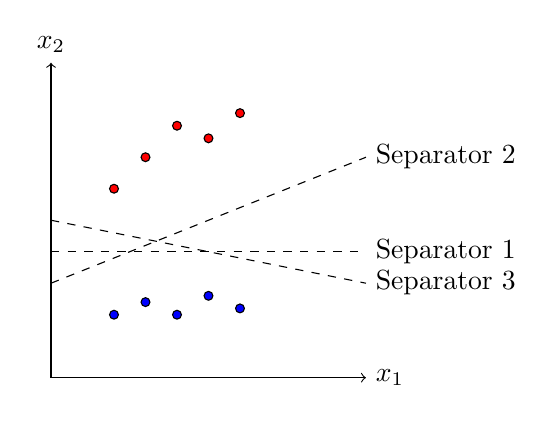
\begin{tikzpicture}[scale=0.8]
    % Coordinate axes
    \draw[->] (0,0) -- (5,0) node[right] {$x_1$};
    \draw[->] (0,0) -- (0,5) node[above] {$x_2$};
    
    % Data points
    \foreach \x/\y in {1/1, 1.5/1.2, 2/1, 2.5/1.3, 3/1.1}
        \draw[fill=blue] (\x,\y) circle (2pt);
    
    \foreach \x/\y in {1/3, 1.5/3.5, 2/4, 2.5/3.8, 3/4.2}
        \draw[fill=red] (\x,\y) circle (2pt);
    
    % Multiple possible decision boundaries
    \draw[dashed] (0,2) -- (5,2) node[right] {Separator 1};
    \draw[dashed] (0,1.5) -- (5,3.5) node[right] {Separator 2};
    \draw[dashed] (0,2.5) -- (5,1.5) node[right] {Separator 3};
\end{tikzpicture}
\caption{Multiple possible linear separators for a linearly separable dataset}
\end{figure}

\section{The Maximum-Margin Approach}

\subsection{The Learning Problem}
Let's formalize the learning problem for linear classification:

Given training data $(\mathbf{x}^{(1)}, y^{(1)}), \ldots, (\mathbf{x}^{(n)}, y^{(n)}) \in \mathbb{R}^d \times \{-1, +1\}$, find $\mathbf{w} \in \mathbb{R}^d$ and $b \in \mathbb{R}$ such that:

\[
y^{(i)}(\mathbf{w} \cdot \mathbf{x}^{(i)} + b) > 0 \quad \text{for all } i = 1, 2, \ldots, n
\]

This condition ensures that all training examples are correctly classified.

\subsection{Scaling the Parameters}
An important observation is that if $(\mathbf{w}, b)$ is a solution to the learning problem, then $(c\mathbf{w}, cb)$ is also a solution for any $c > 0$. This is because:

\[
y^{(i)}(c\mathbf{w} \cdot \mathbf{x}^{(i)} + cb) = c \cdot y^{(i)}(\mathbf{w} \cdot \mathbf{x}^{(i)} + b) > 0
\]

This scaling property allows us to reformulate the problem. We can equivalently ask for:

\[
y^{(i)}(\mathbf{w} \cdot \mathbf{x}^{(i)} + b) \geq 1 \quad \text{for all } i = 1, 2, \ldots, n
\]

This reformulation will be crucial for defining the margin.

\subsection{Defining the Margin}
The margin of a linear classifier is the distance from the decision boundary to the nearest training point. For a linear classifier defined by $\mathbf{w}$ and $b$, the decision boundary is the hyperplane:

\[
\mathbf{w} \cdot \mathbf{x} + b = 0
\]

The constraint $y^{(i)}(\mathbf{w} \cdot \mathbf{x}^{(i)} + b) \geq 1$ implies that:
\begin{itemize}
    \item All positive points ($y^{(i)} = +1$) satisfy $\mathbf{w} \cdot \mathbf{x}^{(i)} + b \geq 1$
    \item All negative points ($y^{(i)} = -1$) satisfy $\mathbf{w} \cdot \mathbf{x}^{(i)} + b \leq -1$
\end{itemize}

This means that all positive points are on or above the hyperplane $\mathbf{w} \cdot \mathbf{x} + b = 1$, and all negative points are on or below the hyperplane $\mathbf{w} \cdot \mathbf{x} + b = -1$.

\begin{figure}[h]
\centering
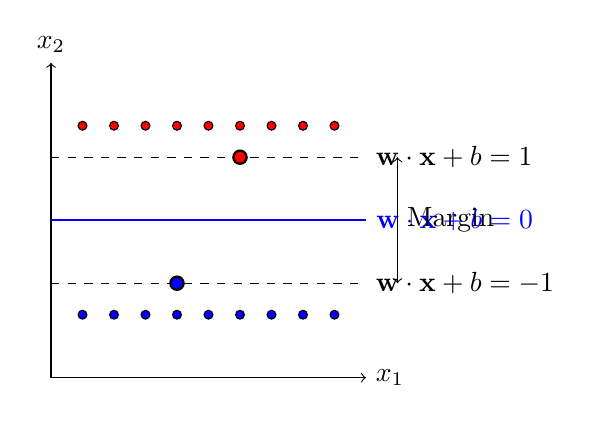
\begin{tikzpicture}[scale=0.8]
    % Coordinate axes
    \draw[->] (0,0) -- (5,0) node[right] {$x_1$};
    \draw[->] (0,0) -- (0,5) node[above] {$x_2$};
    
    % Decision boundary
    \draw[thick, blue] (0,2.5) -- (5,2.5) node[right] {$\mathbf{w} \cdot \mathbf{x} + b = 0$};
    
    % Margin boundaries
    \draw[dashed] (0,1.5) -- (5,1.5) node[right] {$\mathbf{w} \cdot \mathbf{x} + b = -1$};
    \draw[dashed] (0,3.5) -- (5,3.5) node[right] {$\mathbf{w} \cdot \mathbf{x} + b = 1$};
    
    % Margin
    \draw[<->] (5.5,1.5) -- (5.5,3.5) node[midway, right] {Margin};
    
    % Data points
    \foreach \x in {0.5,1,...,4.5}
        \draw[fill=blue] (\x,1) circle (2pt);
    
    \foreach \x in {0.5,1,...,4.5}
        \draw[fill=red] (\x,4) circle (2pt);
    
    % Support vectors
    \draw[fill=blue, thick] (2,1.5) circle (3pt);
    \draw[fill=red, thick] (3,3.5) circle (3pt);
\end{tikzpicture}
\caption{Illustration of the margin in a linearly separable dataset. The support vectors (highlighted) lie exactly on the margin boundaries.}
\end{figure}

\subsection{Calculating the Margin}
The distance from a point $\mathbf{x}$ to the hyperplane $\mathbf{w} \cdot \mathbf{x} + b = 0$ is given by:

\[
\text{distance} = \frac{|\mathbf{w} \cdot \mathbf{x} + b|}{\|\mathbf{w}\|}
\]

For points on the hyperplanes $\mathbf{w} \cdot \mathbf{x} + b = 1$ and $\mathbf{w} \cdot \mathbf{x} + b = -1$, this distance is:

\[
\text{distance} = \frac{1}{\|\mathbf{w}\|}
\]

Therefore, the margin $\gamma$ is:

\[
\gamma = \frac{1}{\|\mathbf{w}\|}
\]

\subsection{Maximizing the Margin}
To maximize the margin $\gamma = \frac{1}{\|\mathbf{w}\|}$, we need to minimize $\|\mathbf{w}\|$. Since minimizing $\|\mathbf{w}\|$ is equivalent to minimizing $\|\mathbf{w}\|^2$ (and the latter is differentiable everywhere), we can formulate the maximum-margin classification problem as:

\[
\min_{\mathbf{w} \in \mathbb{R}^d, b \in \mathbb{R}} \|\mathbf{w}\|^2
\]

subject to:

\[
y^{(i)}(\mathbf{w} \cdot \mathbf{x}^{(i)} + b) \geq 1 \quad \text{for all } i = 1, 2, \ldots, n
\]

This is a convex quadratic optimization problem with linear constraints, which can be solved efficiently using standard optimization techniques.

\section{Support Vector Machines}

\subsection{The Optimization Problem}
The optimization problem for finding the maximum-margin linear classifier is:

\fbox{
\begin{minipage}{\dimexpr\textwidth-2\fboxsep-2\fboxrule\relax}
\textbf{Hard-Margin SVM Optimization Problem}

\begin{align}
\min_{\mathbf{w} \in \mathbb{R}^d, b \in \mathbb{R}} & \|\mathbf{w}\|^2 \\
\text{subject to } & y^{(i)}(\mathbf{w} \cdot \mathbf{x}^{(i)} + b) \geq 1 \quad \text{for all } i = 1, 2, \ldots, n
\end{align}
\end{minipage}
}

This formulation is known as the hard-margin Support Vector Machine (SVM).

\subsection{Properties of the Solution}
The solution to the SVM optimization problem has several important properties:

\begin{itemize}
    \item It is a convex optimization problem, which means that it has a unique global minimum
    \item The solution depends only on a subset of the training points, called support vectors
    \item Support vectors are the points that lie exactly on the margin, i.e., $y^{(i)}(\mathbf{w} \cdot \mathbf{x}^{(i)} + b) = 1$
\end{itemize}

\subsection{Support Vectors}
The solution to the SVM optimization problem can be expressed as:

\[
\mathbf{w} = \sum_{i=1}^{n} \alpha_i y^{(i)} \mathbf{x}^{(i)}
\]

where $\alpha_i \geq 0$ are Lagrange multipliers. Importantly, $\alpha_i > 0$ only for the support vectors (points that lie exactly on the margin). For all other points, $\alpha_i = 0$.

This means that the solution $\mathbf{w}$ is a linear combination of only the support vectors, and the decision boundary is determined entirely by these points.

\begin{figure}[h]
\centering
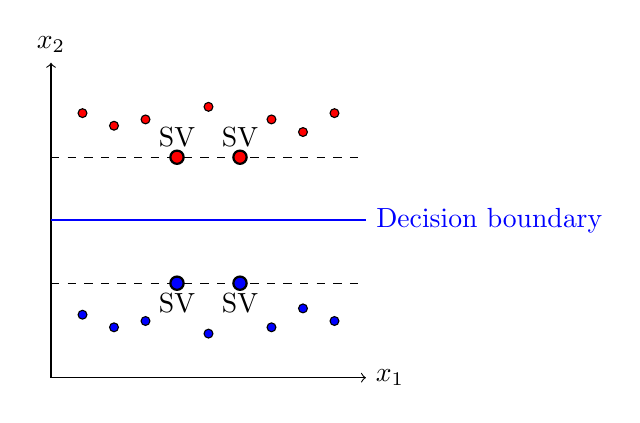
\begin{tikzpicture}[scale=0.8]
    % Coordinate axes
    \draw[->] (0,0) -- (5,0) node[right] {$x_1$};
    \draw[->] (0,0) -- (0,5) node[above] {$x_2$};
    
    % Decision boundary
    \draw[thick, blue] (0,2.5) -- (5,2.5) node[right] {Decision boundary};
    
    % Margin boundaries
    \draw[dashed] (0,1.5) -- (5,1.5);
    \draw[dashed] (0,3.5) -- (5,3.5);
    
    % Data points
    \foreach \x/\y in {0.5/1, 1/0.8, 1.5/0.9, 2.5/0.7, 3.5/0.8, 4/1.1, 4.5/0.9}
        \draw[fill=blue] (\x,\y) circle (2pt);
    
    \foreach \x/\y in {0.5/4.2, 1/4, 1.5/4.1, 2.5/4.3, 3.5/4.1, 4/3.9, 4.5/4.2}
        \draw[fill=red] (\x,\y) circle (2pt);
    
    % Support vectors
    \draw[fill=blue, thick] (2,1.5) circle (3pt) node[below] {SV};
    \draw[fill=blue, thick] (3,1.5) circle (3pt) node[below] {SV};
    \draw[fill=red, thick] (2,3.5) circle (3pt) node[above] {SV};
    \draw[fill=red, thick] (3,3.5) circle (3pt) node[above] {SV};
\end{tikzpicture}
\caption{Support vectors (SV) are the points that lie exactly on the margin boundaries. The decision boundary is determined entirely by these points.}
\end{figure}

\section{The Dual Formulation}

\subsection{Lagrangian Formulation}
To solve the SVM optimization problem, we can use Lagrange multipliers. The Lagrangian is:

\[
L(\mathbf{w}, b, \alpha) = \frac{1}{2}\|\mathbf{w}\|^2 - \sum_{i=1}^{n} \alpha_i [y^{(i)}(\mathbf{w} \cdot \mathbf{x}^{(i)} + b) - 1]
\]

where $\alpha_i \geq 0$ are the Lagrange multipliers.

\subsection{Dual Problem}
By taking derivatives of the Lagrangian with respect to $\mathbf{w}$ and $b$ and setting them to zero, we get:

\[
\mathbf{w} = \sum_{i=1}^{n} \alpha_i y^{(i)} \mathbf{x}^{(i)}
\]

\[
\sum_{i=1}^{n} \alpha_i y^{(i)} = 0
\]

Substituting these back into the Lagrangian, we get the dual problem:

\[
\max_{\alpha} \sum_{i=1}^{n} \alpha_i - \frac{1}{2} \sum_{i=1}^{n} \sum_{j=1}^{n} \alpha_i \alpha_j y^{(i)} y^{(j)} \mathbf{x}^{(i)} \cdot \mathbf{x}^{(j)}
\]

subject to:

\[
\alpha_i \geq 0 \quad \text{for all } i = 1, 2, \ldots, n
\]

\[
\sum_{i=1}^{n} \alpha_i y^{(i)} = 0
\]

This dual formulation is often easier to solve than the primal problem, especially when the number of features is large.

\section{Example: Iris Dataset}

\subsection{Dataset Description}
The Iris dataset is a classic dataset in machine learning, collected by the botanist Edgar Anderson and made famous by the statistician Ronald Fisher. It contains measurements of 150 iris flowers from three different species:

\begin{itemize}
    \item Iris setosa
    \item Iris versicolor
    \item Iris virginica
\end{itemize}

For each flower, four measurements were taken:
\begin{itemize}
    \item Sepal length
    \item Sepal width
    \item Petal length
    \item Petal width
\end{itemize}

\subsection{Binary Classification Example}
For simplicity, let's consider a binary classification problem using only two of the species (setosa and versicolor) and two of the features (sepal width and petal width).

\begin{figure}[h]
\centering
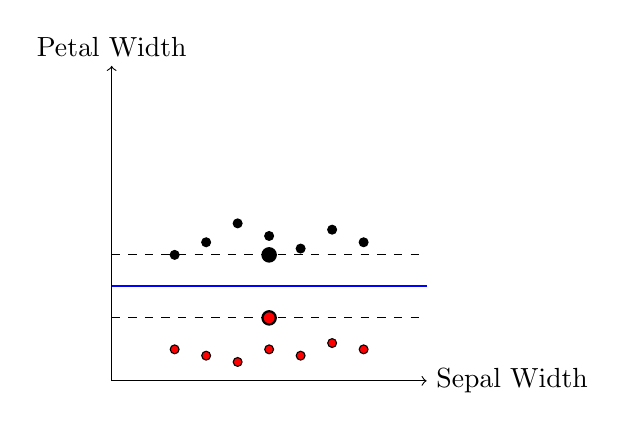
\begin{tikzpicture}[scale=0.8]
    % Coordinate axes
    \draw[->] (0,0) -- (5,0) node[right] {Sepal Width};
    \draw[->] (0,0) -- (0,5) node[above] {Petal Width};
    
    % Setosa (red circles)
    \foreach \x/\y in {1/0.5, 1.5/0.4, 2/0.3, 2.5/0.5, 3/0.4, 3.5/0.6, 4/0.5}
        \draw[fill=red] (\x,\y) circle (2pt);
    
    % Versicolor (black triangles)
    \foreach \x/\y in {1/2, 1.5/2.2, 2/2.5, 2.5/2.3, 3/2.1, 3.5/2.4, 4/2.2}
        \draw[fill=black] (\x,\y) circle (2pt);
    
    % Decision boundary
    \draw[thick, blue] (0,1.5) -- (5,1.5);
    
    % Margin boundaries
    \draw[dashed] (0,1) -- (5,1);
    \draw[dashed] (0,2) -- (5,2);
    
    % Support vectors
    \draw[fill=red, thick] (2.5,1) circle (3pt);
    \draw[fill=black, thick] (2.5,2) circle (3pt);
\end{tikzpicture}
\caption{SVM classification of Iris setosa (red circles) and Iris versicolor (black triangles) using sepal width and petal width features.}
\end{figure}

In this example, the data is linearly separable, and the SVM finds the maximum-margin linear classifier. The support vectors are the points that lie exactly on the margin boundaries.

\section{Soft-Margin SVM}

\subsection{Handling Non-linearly Separable Data}
The hard-margin SVM assumes that the data is linearly separable. However, in real-world scenarios, data is often not perfectly separable due to noise or outliers. To handle such cases, we can use a soft-margin SVM, which allows for some misclassifications.

\subsection{Slack Variables}
We introduce slack variables $\xi_i \geq 0$ for each training point, which measure the degree of misclassification:

\[
y^{(i)}(\mathbf{w} \cdot \mathbf{x}^{(i)} + b) \geq 1 - \xi_i \quad \text{for all } i = 1, 2, \ldots, n
\]

If $\xi_i = 0$, the point is correctly classified and on or beyond the margin.
If $0 < \xi_i \leq 1$, the point is correctly classified but within the margin.
If $\xi_i > 1$, the point is misclassified.

\subsection{Optimization Problem}
The soft-margin SVM optimization problem is:

\fbox{
\begin{minipage}{\dimexpr\textwidth-2\fboxsep-2\fboxrule\relax}
\textbf{Soft-Margin SVM Optimization Problem}

\begin{align}
\min_{\mathbf{w}, b, \xi} & \frac{1}{2}\|\mathbf{w}\|^2 + C \sum_{i=1}^{n} \xi_i \\
\text{subject to } & y^{(i)}(\mathbf{w} \cdot \mathbf{x}^{(i)} + b) \geq 1 - \xi_i \quad \text{for all } i = 1, 2, \ldots, n \\
& \xi_i \geq 0 \quad \text{for all } i = 1, 2, \ldots, n
\end{align}
\end{minipage}
}

The parameter $C > 0$ controls the trade-off between maximizing the margin and minimizing the classification error. A larger $C$ places more emphasis on correctly classifying all training points, while a smaller $C$ places more emphasis on maximizing the margin.

\begin{figure}[h]
\centering
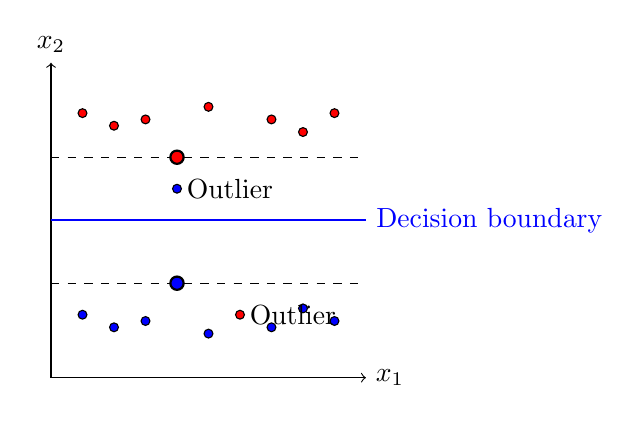
\begin{tikzpicture}[scale=0.8]
    % Coordinate axes
    \draw[->] (0,0) -- (5,0) node[right] {$x_1$};
    \draw[->] (0,0) -- (0,5) node[above] {$x_2$};
    
    % Decision boundary
    \draw[thick, blue] (0,2.5) -- (5,2.5) node[right] {Decision boundary};
    
    % Margin boundaries
    \draw[dashed] (0,1.5) -- (5,1.5);
    \draw[dashed] (0,3.5) -- (5,3.5);
    
    % Data points
    \foreach \x/\y in {0.5/1, 1/0.8, 1.5/0.9, 2.5/0.7, 3.5/0.8, 4/1.1, 4.5/0.9}
        \draw[fill=blue] (\x,\y) circle (2pt);
    
    \foreach \x/\y in {0.5/4.2, 1/4, 1.5/4.1, 2.5/4.3, 3.5/4.1, 4/3.9, 4.5/4.2}
        \draw[fill=red] (\x,\y) circle (2pt);
    
    % Outliers
    \draw[fill=blue] (2,3) circle (2pt) node[right] {Outlier};
    \draw[fill=red] (3,1) circle (2pt) node[right] {Outlier};
    
    % Support vectors
    \draw[fill=blue, thick] (2,1.5) circle (3pt);
    \draw[fill=red, thick] (2,3.5) circle (3pt);
\end{tikzpicture}
\caption{Soft-margin SVM allows for some misclassifications to handle outliers or non-linearly separable data.}
\end{figure}

\section{Kernel Methods for Non-linear Classification}

\subsection{Limitations of Linear Classifiers}
Linear classifiers, including hard-margin and soft-margin SVMs, can only learn linear decision boundaries. However, many real-world datasets require non-linear decision boundaries for effective classification.

\begin{figure}[h]
\centering
\begin{tikzpicture}[scale=0.8]
    % Coordinate axes
    \draw[->] (0,0) -- (5,0) node[right] {$x_1$};
    \draw[->] (0,0) -- (0,5) node[above] {$x_2$};
    
    % Data points - XOR pattern
    \draw[fill=red] (1,1) circle (2pt);
    \draw[fill=red] (4,4) circle (2pt);
    \draw[fill=blue] (1,4) circle (2pt);
    \draw[fill=blue] (4,1) circle (2pt);
    
    % Non-linear decision boundary
    \draw[thick, blue] (2.5,0) arc (0:180:2.5);
    \draw[thick, blue] (2.5,0) arc (0:180:2.5 and 1.25);
    \draw[thick, blue] (2.5,5) arc (180:360:2.5 and 1.25);
\end{tikzpicture}
\caption{Example of data that requires a non-linear decision boundary (XOR pattern)}
\end{figure}

\subsection{The Kernel Trick}
The kernel trick is a clever technique that allows SVMs to learn non-linear decision boundaries without explicitly mapping the data to a higher-dimensional space. It relies on the observation that the dual formulation of the SVM optimization problem only depends on inner products between data points.

\subsubsection{Feature Maps}
Let $\phi: \mathbb{R}^d \rightarrow \mathbb{R}^D$ be a feature map that maps data from the original $d$-dimensional space to a higher-dimensional space $\mathbb{R}^D$. The idea is to find a linear boundary in this higher-dimensional space, which corresponds to a non-linear boundary in the original space.

\subsubsection{Kernel Functions}
A kernel function $K: \mathbb{R}^d \times \mathbb{R}^d \rightarrow \mathbb{R}$ computes the inner product in the higher-dimensional space without explicitly computing the mapping:

\[
K(\mathbf{x}, \mathbf{z}) = \phi(\mathbf{x}) \cdot \phi(\mathbf{z})
\]

This is powerful because:
\begin{itemize}
    \item We never need to explicitly compute $\phi(\mathbf{x})$, which could be very high-dimensional or even infinite-dimensional
    \item We only need to define the kernel function $K$, which computes the inner product directly
\end{itemize}

\subsection{Common Kernel Functions}
Several kernel functions are commonly used in practice:

\begin{itemize}
    \item \textbf{Linear kernel}: $K(\mathbf{x}, \mathbf{z}) = \mathbf{x} \cdot \mathbf{z}$
    \item \textbf{Polynomial kernel}: $K(\mathbf{x}, \mathbf{z}) = (\mathbf{x} \cdot \mathbf{z} + c)^d$, where $c \geq 0$ and $d \in \mathbb{N}$
    \item \textbf{Radial Basis Function (RBF) kernel}: $K(\mathbf{x}, \mathbf{z}) = \exp(-\gamma \|\mathbf{x} - \mathbf{z}\|^2)$, where $\gamma > 0$
    \item \textbf{Sigmoid kernel}: $K(\mathbf{x}, \mathbf{z}) = \tanh(\alpha \mathbf{x} \cdot \mathbf{z} + c)$, where $\alpha > 0$ and $c \geq 0$
\end{itemize}

\subsection{Kernel SVM Formulation}
The dual formulation of the SVM optimization problem with kernels is:

\[
\max_{\alpha} \sum_{i=1}^{n} \alpha_i - \frac{1}{2} \sum_{i=1}^{n} \sum_{j=1}^{n} \alpha_i \alpha_j y^{(i)} y^{(j)} K(\mathbf{x}^{(i)}, \mathbf{x}^{(j)})
\]

subject to:

\[
\alpha_i \geq 0 \quad \text{for all } i = 1, 2, \ldots, n
\]

\[
\sum_{i=1}^{n} \alpha_i y^{(i)} = 0
\]

The decision function becomes:

\[
f(\mathbf{x}) = \text{sign}\left(\sum_{i=1}^{n} \alpha_i y^{(i)} K(\mathbf{x}^{(i)}, \mathbf{x}) + b\right)
\]

\subsection{Example: RBF Kernel}
The RBF kernel is particularly popular because it can model complex non-linear decision boundaries. It effectively measures the similarity between two points based on their Euclidean distance:

\[
K(\mathbf{x}, \mathbf{z}) = \exp(-\gamma \|\mathbf{x} - \mathbf{z}\|^2)
\]

The parameter $\gamma$ controls the "width" of the kernel:
\begin{itemize}
    \item Small $\gamma$: Wide kernel, smooth decision boundary
    \item Large $\gamma$: Narrow kernel, more complex decision boundary
\end{itemize}

\begin{figure}[h]
\centering
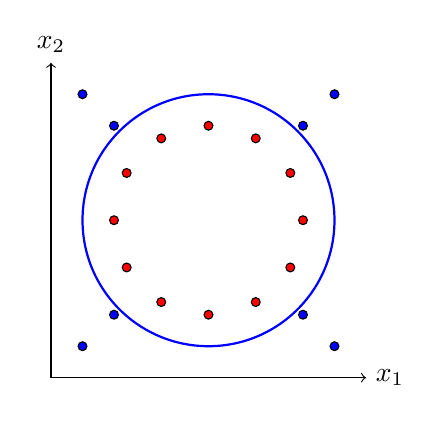
\begin{tikzpicture}[scale=0.8]
    % Coordinate axes
    \draw[->] (0,0) -- (5,0) node[right] {$x_1$};
    \draw[->] (0,0) -- (0,5) node[above] {$x_2$};
    
    % Data points - circular pattern
    \foreach \angle in {0,30,...,330}
        \draw[fill=red] ({2.5+1.5*cos(\angle)},{2.5+1.5*sin(\angle)}) circle (2pt);
    
    \foreach \x/\y in {0.5/0.5, 0.5/4.5, 4.5/0.5, 4.5/4.5, 1/1, 1/4, 4/1, 4/4}
        \draw[fill=blue] (\x,\y) circle (2pt);
    
    % Non-linear decision boundary
    \draw[thick, blue] (2.5,2.5) circle (2);
\end{tikzpicture}
\caption{Example of a non-linear decision boundary learned using an RBF kernel}
\end{figure}

\section{Multi-class SVMs}

\subsection{Extending SVMs to Multiple Classes}
SVMs are inherently binary classifiers, but many real-world problems involve multiple classes. Several strategies exist for extending SVMs to multi-class classification:

\subsubsection{One-vs-Rest (OVR)}
In the One-vs-Rest approach:
\begin{itemize}
    \item Train $k$ binary SVMs, where $k$ is the number of classes
    \item Each SVM distinguishes one class from all other classes
    \item For a new point, evaluate all $k$ SVMs and assign the class with the highest confidence score
\end{itemize}

\begin{figure}[h]
\centering
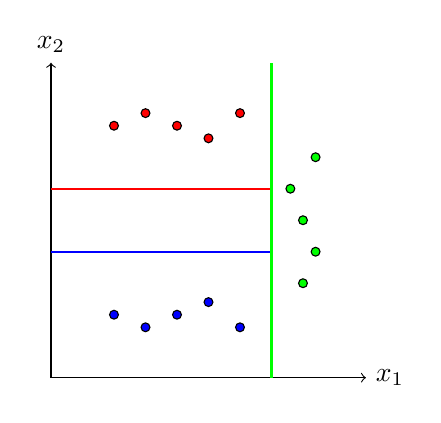
\begin{tikzpicture}[scale=0.8]
    % Coordinate axes
    \draw[->] (0,0) -- (5,0) node[right] {$x_1$};
    \draw[->] (0,0) -- (0,5) node[above] {$x_2$};
    
    % Class 1 (red)
    \foreach \x/\y in {1/4, 1.5/4.2, 2/4, 2.5/3.8, 3/4.2}
        \draw[fill=red] (\x,\y) circle (2pt);
    
    % Class 2 (blue)
    \foreach \x/\y in {1/1, 1.5/0.8, 2/1, 2.5/1.2, 3/0.8}
        \draw[fill=blue] (\x,\y) circle (2pt);
    
    % Class 3 (green)
    \foreach \x/\y in {4/2.5, 4.2/2, 4/1.5, 3.8/3, 4.2/3.5}
        \draw[fill=green] (\x,\y) circle (2pt);
    
    % Decision boundaries
    \draw[thick, red] (0,3) -- (3.5,3) -- (3.5,5);
    \draw[thick, blue] (0,2) -- (3.5,2) -- (3.5,0);
    \draw[thick, green] (3.5,0) -- (3.5,5);
\end{tikzpicture}
\caption{One-vs-Rest approach for multi-class SVM with three classes}
\end{figure}

\subsubsection{One-vs-One (OVO)}
In the One-vs-One approach:
\begin{itemize}
    \item Train $\binom{k}{2} = \frac{k(k-1)}{2}$ binary SVMs, one for each pair of classes
    \item For a new point, each binary SVM votes for one class
    \item Assign the class with the most votes
\end{itemize}

\begin{figure}[h]
\centering
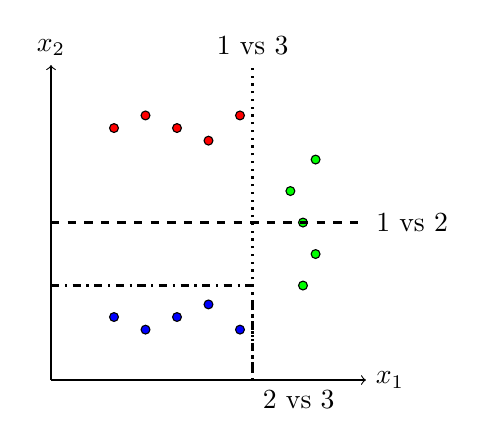
\begin{tikzpicture}[scale=0.8]
    % Coordinate axes
    \draw[->] (0,0) -- (5,0) node[right] {$x_1$};
    \draw[->] (0,0) -- (0,5) node[above] {$x_2$};
    
    % Class 1 (red)
    \foreach \x/\y in {1/4, 1.5/4.2, 2/4, 2.5/3.8, 3/4.2}
        \draw[fill=red] (\x,\y) circle (2pt);
    
    % Class 2 (blue)
    \foreach \x/\y in {1/1, 1.5/0.8, 2/1, 2.5/1.2, 3/0.8}
        \draw[fill=blue] (\x,\y) circle (2pt);
    
    % Class 3 (green)
    \foreach \x/\y in {4/2.5, 4.2/2, 4/1.5, 3.8/3, 4.2/3.5}
        \draw[fill=green] (\x,\y) circle (2pt);
    
    % Decision boundaries
    \draw[thick, dashed] (0,2.5) -- (5,2.5) node[right] {1 vs 2};
    \draw[thick, dotted] (3.2,0) -- (3.2,5) node[above] {1 vs 3};
    \draw[thick, dashdotted] (0,1.5) -- (3.2,1.5) -- (3.2,0) node[below right] {2 vs 3};
\end{tikzpicture}
\caption{One-vs-One approach for multi-class SVM with three classes}
\end{figure}

\subsubsection{Direct Multi-class Formulation}
There are also direct formulations of multi-class SVMs that solve a single optimization problem:
\begin{itemize}
    \item Crammer and Singer's multi-class SVM
    \item Weston and Watkins' multi-class SVM
\end{itemize}

These formulations are more complex but can sometimes yield better results than the OVR or OVO approaches.

\subsection{Comparison of Multi-class Strategies}
\begin{itemize}
    \item \textbf{One-vs-Rest}:
    \begin{itemize}
        \item Pros: Simple, only requires $k$ classifiers
        \item Cons: Class imbalance, ambiguous regions
    \end{itemize}
    \item \textbf{One-vs-One}:
    \begin{itemize}
        \item Pros: Better handling of class imbalance, smaller training sets for each classifier
        \item Cons: Requires $\binom{k}{2}$ classifiers, which can be large for many classes
    \end{itemize}
    \item \textbf{Direct Multi-class}:
    \begin{itemize}
        \item Pros: Theoretically more principled, considers all classes simultaneously
        \item Cons: More complex optimization problem, computationally expensive
    \end{itemize}
\end{itemize}

\section{Practical Considerations}

\subsection{Hyperparameter Selection}
SVMs have several hyperparameters that need to be tuned:
\begin{itemize}
    \item $C$: The regularization parameter in soft-margin SVMs
    \item Kernel parameters (e.g., $\gamma$ in RBF kernel, $d$ in polynomial kernel)
\end{itemize}

These hyperparameters are typically selected using cross-validation:
\begin{itemize}
    \item Split the data into training and validation sets
    \item Train SVMs with different hyperparameter values on the training set
    \item Evaluate performance on the validation set
    \item Select the hyperparameters that yield the best validation performance
\end{itemize}

\subsection{Feature Scaling}
SVMs are sensitive to the scale of the features. It's generally recommended to scale the features before training an SVM:
\begin{itemize}
    \item Standardization: $x' = \frac{x - \mu}{\sigma}$
    \item Min-max scaling: $x' = \frac{x - \min(x)}{\max(x) - \min(x)}$
\end{itemize}

\subsection{Handling Large Datasets}
Standard SVM implementations have time complexity $O(n^2)$ to $O(n^3)$, where $n$ is the number of training examples. This can be prohibitive for large datasets. Several approaches exist for scaling SVMs to large datasets:
\begin{itemize}
    \item Chunking: Solve the optimization problem in smaller chunks
    \item Sequential Minimal Optimization (SMO): Optimize two Lagrange multipliers at a time
    \item Stochastic gradient descent: Approximate the SVM solution using SGD
    \item Linear SVMs: For linear kernels, specialized algorithms like LIBLINEAR can scale to millions of examples
\end{itemize}

\subsection{Probabilistic Outputs}
Standard SVMs output only the class label, not a probability. However, there are methods to convert SVM outputs to probabilities:
\begin{itemize}
    \item Platt scaling: Fit a logistic regression model to the SVM scores
    \item Isotonic regression: A more flexible non-parametric approach
\end{itemize}

\section{Worked Examples}

\subsection{Example 1: Linear SVM on a 2D Dataset}
Consider a simple 2D dataset with two classes:
\begin{itemize}
    \item Positive examples: $(1,1)$, $(2,3)$, $(3,2)$
    \item Negative examples: $(1,3)$, $(2,1)$, $(3,3)$
\end{itemize}

\begin{figure}[h]
\centering
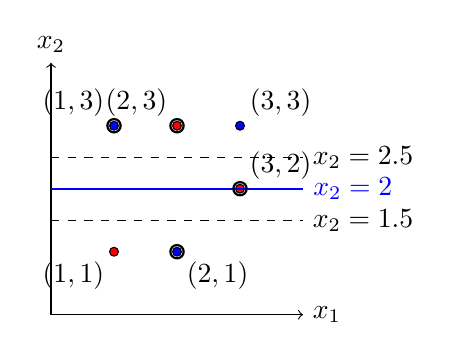
\begin{tikzpicture}[scale=0.8]
    % Coordinate axes
    \draw[->] (0,0) -- (4,0) node[right] {$x_1$};
    \draw[->] (0,0) -- (0,4) node[above] {$x_2$};
    
    % Data points
    \draw[fill=red] (1,1) circle (2pt) node[below left] {$(1,1)$};
    \draw[fill=red] (2,3) circle (2pt) node[above left] {$(2,3)$};
    \draw[fill=red] (3,2) circle (2pt) node[above right] {$(3,2)$};
    \draw[fill=blue] (1,3) circle (2pt) node[above left] {$(1,3)$};
    \draw[fill=blue] (2,1) circle (2pt) node[below right] {$(2,1)$};
    \draw[fill=blue] (3,3) circle (2pt) node[above right] {$(3,3)$};
    
    % Decision boundary
    \draw[thick, blue] (0,2) -- (4,2) node[right] {$x_2 = 2$};
    
    % Margin boundaries
    \draw[dashed] (0,1.5) -- (4,1.5) node[right] {$x_2 = 1.5$};
    \draw[dashed] (0,2.5) -- (4,2.5) node[right] {$x_2 = 2.5$};
    
    % Support vectors
    \draw[thick] (2,1) circle (3pt);
    \draw[thick] (3,2) circle (3pt);
    \draw[thick] (1,3) circle (3pt);
    \draw[thick] (2,3) circle (3pt);
\end{tikzpicture}
\caption{Linear SVM on a 2D dataset. The decision boundary is $x_2 = 2$, and the support vectors are circled.}
\end{figure}

The SVM finds the decision boundary $x_2 = 2$, which corresponds to $w = (0, 1)$ and $b = -2$. The margin is $\gamma = 1/\|w\| = 1$, and the support vectors are the points closest to the decision boundary: $(2,1)$, $(3,2)$, $(1,3)$, and $(2,3)$.

\subsection{Example 2: Soft-Margin SVM with Outliers}
Now, let's add an outlier to the dataset:
\begin{itemize}
    \item Positive examples: $(1,1)$, $(2,3)$, $(3,2)$, $(2,0.5)$ (outlier)
    \item Negative examples: $(1,3)$, $(2,1)$, $(3,3)$
\end{itemize}

\begin{figure}[h]
\centering
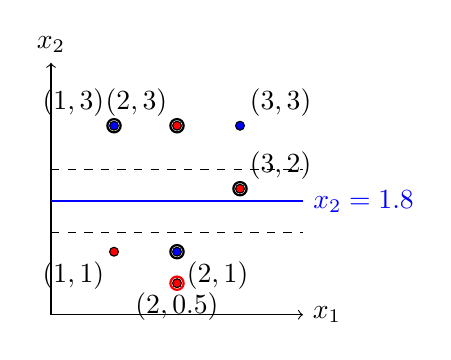
\begin{tikzpicture}[scale=0.8]
    % Coordinate axes
    \draw[->] (0,0) -- (4,0) node[right] {$x_1$};
    \draw[->] (0,0) -- (0,4) node[above] {$x_2$};
    
    % Data points
    \draw[fill=red] (1,1) circle (2pt) node[below left] {$(1,1)$};
    \draw[fill=red] (2,3) circle (2pt) node[above left] {$(2,3)$};
    \draw[fill=red] (3,2) circle (2pt) node[above right] {$(3,2)$};
    \draw[fill=red] (2,0.5) circle (2pt) node[below] {$(2,0.5)$};
    \draw[fill=blue] (1,3) circle (2pt) node[above left] {$(1,3)$};
    \draw[fill=blue] (2,1) circle (2pt) node[below right] {$(2,1)$};
    \draw[fill=blue] (3,3) circle (2pt) node[above right] {$(3,3)$};
    
    % Decision boundary
    \draw[thick, blue] (0,1.8) -- (4,1.8) node[right] {$x_2 = 1.8$};
    
    % Margin boundaries
    \draw[dashed] (0,1.3) -- (4,1.3);
    \draw[dashed] (0,2.3) -- (4,2.3);
    
    % Support vectors
    \draw[thick] (2,1) circle (3pt);
    \draw[thick] (3,2) circle (3pt);
    \draw[thick] (1,3) circle (3pt);
    \draw[thick] (2,3) circle (3pt);
    
    % Outlier
    \draw[thick, red] (2,0.5) circle (3pt);
\end{tikzpicture}
\caption{Soft-margin SVM with an outlier. The decision boundary shifts slightly to accommodate the outlier.}
\end{figure}

With a hard-margin SVM, this dataset would not be linearly separable due to the outlier. However, a soft-margin SVM can handle the outlier by allowing it to be misclassified (with a penalty determined by the parameter $C$).

\subsection{Example 3: Non-linear SVM with RBF Kernel}
Consider a dataset with a circular pattern:
\begin{itemize}
    \item Positive examples: Points inside a circle
    \item Negative examples: Points outside the circle
\end{itemize}

\begin{figure}[h]
\centering
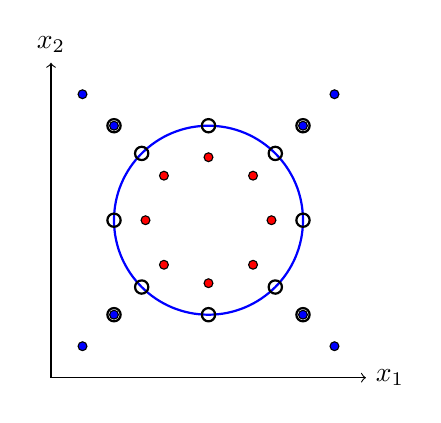
\begin{tikzpicture}[scale=0.8]
    % Coordinate axes
    \draw[->] (0,0) -- (5,0) node[right] {$x_1$};
    \draw[->] (0,0) -- (0,5) node[above] {$x_2$};
    
    % Circle
    \draw[thick, blue] (2.5,2.5) circle (1.5);
    
    % Points inside the circle (positive)
    \foreach \angle in {0,45,...,315}
        \draw[fill=red] ({2.5+cos(\angle)},{2.5+sin(\angle)}) circle (2pt);
    
    % Points outside the circle (negative)
    \foreach \x/\y in {0.5/0.5, 0.5/4.5, 4.5/0.5, 4.5/4.5, 1/1, 1/4, 4/1, 4/4}
        \draw[fill=blue] (\x,\y) circle (2pt);
    
    % Support vectors
    \foreach \angle in {0,45,...,315}
        \draw[thick] ({2.5+1.5*cos(\angle)},{2.5+1.5*sin(\angle)}) circle (3pt);
    
    \foreach \x/\y in {1/1, 1/4, 4/1, 4/4}
        \draw[thick] (\x,\y) circle (3pt);
\end{tikzpicture}
\caption{Non-linear SVM with RBF kernel. The decision boundary is a circle, and the support vectors are circled.}
\end{figure}

This dataset is not linearly separable, but an SVM with an RBF kernel can learn the circular decision boundary. The support vectors are the points closest to the decision boundary.

\section{Summary and Key Takeaways}

\subsection{Core Concepts}
\begin{itemize}
    \item Support Vector Machines (SVMs) find the linear classifier with the maximum margin between classes
    \item The margin is the distance from the decision boundary to the nearest training points
    \item Maximizing the margin leads to better generalization to unseen data
    \item The optimization problem for hard-margin SVMs is to minimize $\|w\|^2$ subject to $y^{(i)}(w \cdot x^{(i)} + b) \geq 1$ for all training points
\end{itemize}

\subsection{Extensions}
\begin{itemize}
    \item Soft-margin SVMs allow for some misclassifications to handle non-linearly separable data
    \item Kernel SVMs use the kernel trick to learn non-linear decision boundaries
    \item Multi-class SVMs extend binary SVMs to handle multiple classes
\end{itemize}

\subsection{Strengths of SVMs}
\begin{itemize}
    \item Effective in high-dimensional spaces
    \item Memory efficient (only support vectors are needed for prediction)
    \item Versatile (different kernel functions for different types of data)
    \item Robust to overfitting, especially in high-dimensional spaces
\end{itemize}

\subsection{Limitations of SVMs}
\begin{itemize}
    \item Computationally intensive for large datasets
    \item Sensitive to the choice of kernel and hyperparameters
    \item No direct probability estimates (though methods exist to convert scores to probabilities)
    \item Can be challenging to interpret, especially with non-linear kernels
\end{itemize}

\subsection{Practical Tips}
\begin{itemize}
    \item Scale features before training SVMs
    \item Use cross-validation to select hyperparameters
    \item Start with a linear kernel and move to more complex kernels if needed
    \item For large datasets, consider specialized implementations or approximations
\end{itemize}

\subsection{Connections to Other Methods}
\begin{itemize}
    \item SVMs are related to logistic regression, but focus on the margin rather than probabilistic interpretation
    \item The kernel trick used in SVMs is also applicable to other methods (e.g., kernel PCA, kernel k-means)
    \item SVMs can be viewed as a special case of regularized empirical risk minimization
    \item The concept of maximum margin has influenced other methods, such as boosting algorithms
\end{itemize}

\end{document}